%!TEX root = ../Thesis.tex

%%%%%%%%%%%%%%%%%%%%%%%%%%%%%%%%%%%%%%%%%%%%%%%%%%%%%%%%%%%%%%%%%%%%%%%%
\chapter{Method}
\label{sec:method}

In this chapter, we use the concepts previously described in \autoref{sec:fundamentals} to outline how our algorithm works. It is divided into the search for the correct algorithm and the modifications that lead to our desired result. It also contains the optimization of the algorithm and the visualization of the final result.
%%%%%%%%%%%%%%%%%%%%%%%%%%%%%%%%%%%%%%%%%%%%%%%%%%%%%%%%%%%%%%%%%%%%%%%%

%%%%%%%%%%%%%%%%%%%%%%%%%%%%%%%%%%%%%%%%%%%%%%%%%%%%%%%%%%%%%%%%%%%%%%%%
\section{Motivation}
\label{sec:motivation}
The motivation for this topic stems from the challenging and intriguing idea of using a natural process to solve a computer science problem. The notion of this came as an afterthought of a seminar, in which two edge bundling papers (Winding Roads \cite{lambert_winding_2010} and Edge-Path Bundling \cite{wallinger_edge-path_2022} were discussed. The apparent problem is that Edge-Path Bundling and many other edge bundling algorithms lack a mathematical structure. This lack gave us the idea to use a Steiner tree as a base for the bundling. The Steiner tree also has other beneficial attributes to path bundling. As the tree connects all nodes with the minimal distance between them, and the Steiner points are at the Fermat points, the resulting bundle results in dramatically reduced clutter and a graph whose readability is improved as node-edge overlaps are reduced. 

Despite the existence of other, faster approximation algorithms for Steiner trees like SCIP-Jack \cite{RehfeldtKoch2023}, we decided to use a Physarium Polycephalum approximation algorithm to approximate the Steiner tree. The Physarium algorithm gives us a sound basis for further graph bundling, where we can use the calculation without needing post-processing. The faster calculation was not feasible in the scope of this work; instead, we used the Steiner tree as a routing structure for graph paths. These are ideal for edge bundling as they reduce the size of the graph to a minimum while still connecting all edges and also enable good readability. 
%%%%%%%%%%%%%%%%%%%%%%%%%%%%%%%%%%%%%%%%%%%%%%%%%%%%%%%%%%%%%%%%%%%%%%%%

%%%%%%%%%%%%%%%%%%%%%%%%%%%%%%%%%%%%%%%%%%%%%%%%%%%%%%%%%%%%%%%%%%%%%%%%
\section{Different Approaches of Calculating a Steiner Tree}
\label{sec:different_approaches}

Throughout this thesis, we tried different approaches to calculate a Steiner tree. In the following section, we want to present each method and discuss why we choose it and what benefits or drawbacks each has.

%%%%%%%%%%%%%%%%%%%%%%%%%%%%%%%%%%%%%%%%%%%%%%%%%%%%%%%%%%%%%%%%%%%%%%%%
\subsection{Agent Based Physarium Simulation}
\label{sec:agent-based_approach}

\begin{figure}[t]
    \centering
    \begin{subfigure}{0.45\linewidth}
        \centering
        \includegraphics[width=\linewidth]{figures/agent_plots/simulation_t250_1.png}
        \caption{}
        \label{fig:jeff_0}
    \end{subfigure}
    \begin{subfigure}{0.45\linewidth}
        \centering
        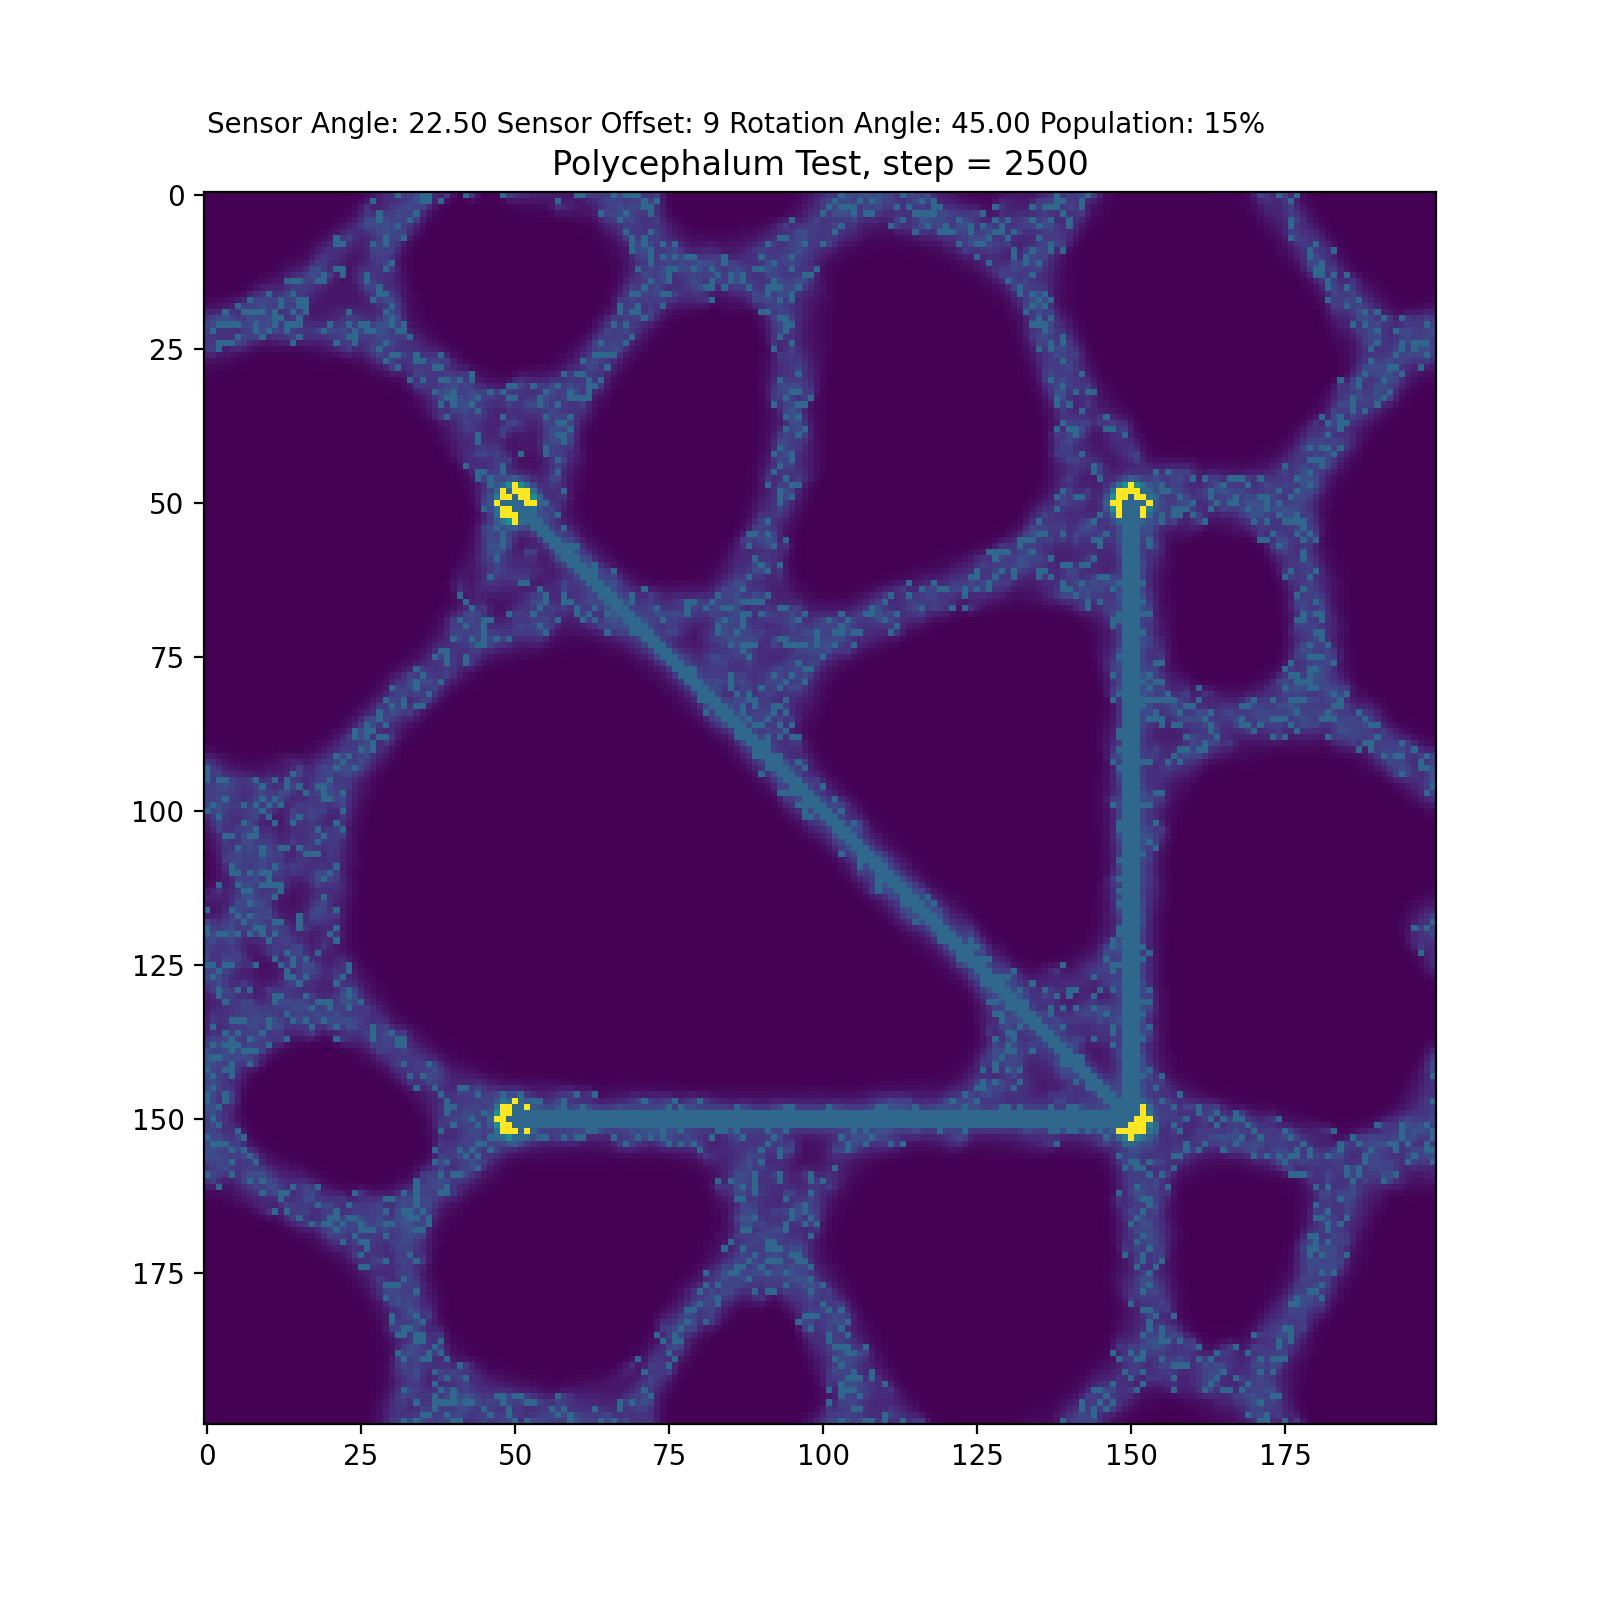
\includegraphics[width=\linewidth]{figures/agent_plots/simulation_t2499.png}
        \caption{}
        \label{fig:jeff_1}
    \end{subfigure}
  \caption{\subref{fig:jeff_0} 250 iterations with five nodes and 165 agents; \subref{fig:jeff_1} 2500 iterations with edges already present for bundling direction.}
  \label{fig:agent_plots}
\end{figure}

At first, we used an agent-based algorithm by Jones et al. \cite{jones_characteristics_2010}. The agents that are used in this approach follow two simple rules based on chemotaxis:

\begin{itemize}
    \item [1.] Deposit trail that diffuses over time
    \item [2.] Sense trails that are left behind by other agents and move in the direction in which the trail is strongest
\end{itemize}

Given enough iterations, the agents form complex patterns that merge into efficient networks. An example network can be seen in \autoref{fig:jeff_0}. We encountered two problems early on. The first was that the patterns were not stable. We tried to mitigate this problem by introducing predetermined paths for a more stable result, as seen in \autoref{fig:jeff_1}. Still, the second problem was that extracting the resulting network efficiently and retaining its accuracy was not feasible. 
%%%%%%%%%%%%%%%%%%%%%%%%%%%%%%%%%%%%%%%%%%%%%%%%%%%%%%%%%%%%%%%%%%%%%%%%

%%%%%%%%%%%%%%%%%%%%%%%%%%%%%%%%%%%%%%%%%%%%%%%%%%%%%%%%%%%%%%%%%%%%%%%%
\subsection{Biology-Inspired Steiner Tree Algorithm}
\label{sec:biology_approach}

We found a paper by Liu et al. \cite{liu_physarum_2015} for the following approach. They stimulate the cytoplasmic flow in the Polycephalum tubes by using the network Poisson equation described in \autoref{sec:physariumPolycephalum}. They discretized the graph onto a grid to find the Steiner points of a graph. The terminals then become an inflow or outflow. Each node contains a list of all combinations of inflows and outflows, and at each iteration, the conductivity and the pressure for each combination are calculated. The edge is cut from the graph if the conductivity is smaller than a threshold. For the pressure update, they use \autoref{eqn:continues_pressure_eqn}, where $p_{i,k}^t$ denotes the pressure at vertex $i$ at iteration step $t$, and $r_k$ is the sink node. 

\begingroup
\large
\begin{equation}
    \label{eqn:continues_pressure_eqn}
    p_{i,k}^{t+1} \approx \begin{cases}
        \frac{I_0 + \sum\limits_{v_j \in N_i} D_{i,j}^{i+1}(p_{i,k}^t + p_{j,k}^t)}{2 \sum\limits_{v_j \in N_i}}, \text{ for } v_i \in T \backslash \{r_k\}; \\
        0, \text{ for } v_i = r_k; \\
        \frac{\sum\limits_{v_j \in N_i} D_{i,j}^{i+1}(p_{i,k}^t + p_{j,k}^t)}{2 \sum\limits_{v_j \in N_i}}, \text{ for } v_i \notin T
    \end{cases}
\end{equation}
\endgroup

The problem with this approach was that they defined points outside the grid, calculated the edge cost concerning these points, and found the best path around them. This was no viable solution for us, as we had to find the overall shortest route in the graph independent from specific points. We also had some problems tuning the parameters to work with our approach.
%%%%%%%%%%%%%%%%%%%%%%%%%%%%%%%%%%%%%%%%%%%%%%%%%%%%%%%%%%%%%%%%%%%%%%%%

%%%%%%%%%%%%%%%%%%%%%%%%%%%%%%%%%%%%%%%%%%%%%%%%%%%%%%%%%%%%%%%%%%%%%%%%
\subsection{Node Weighted Steiner Tree Algorithm}
\label{sec:node_weighted_approach}

The third paper \cite{sun_fast_2016} takes the same approach as the second one by simulation the cytoplasmic flow with the network Poisson equation. The difference is that the node weight and the edge cost are both considered in the equation. Sun et al. used the same flux equation noted in \autoref{eqn:flux} and calculated the composite cost $C(i,j)$ for each edge. $w_i$ are the node weights, $d_i$ the degree and $M$ the maximal weight of all nodes.

\begin{equation}
    \label{eqn:composite_cost_eqn}
    C(i,j) = c_{ij} - \frac{w_i}{d_i} - \frac{w_j}{d_j} + 2M
\end{equation}

They also do not work with the pressure combination to calculate the conductivity. Instead, they use a probability equation to choose the sink node. They then sort the cost in ascending order and select a terminal using $P(i)$. $l(i)$ is the total cost of all edges connected to terminal $i$. $l(i)$ is the total cost of all edges combined.

\begin{equation}
    \label{eqn:probability_eqn}
    P(i) = \frac{l(T-i+1)}{\sum\limits_{j = 1}^Tl(j)}
\end{equation}

The pressure at each vertex is calculated using \autoref{eqn:poisson_eqn}, and the flux is calculated with \autoref{eqn:flux}. After the flux calculation, the conductivity $D_{ij}(k+1)$ needs to be updated. $\alpha_{ij}$ is a positive variable for each edge, $\mu$ a constant and the function $f$ is defined as an increasing function with $f(0) = 0$, and $f(|Q_{ij}(k)|) = \alpha |Q_{ij}(k)|$ and $\alpha$ is another positive variable.

\begin{equation}
    \label{eqn:conductivity_update_eqn}
    D_{ij}(k+1) = \alpha_{ij} \cdot [D_{ij}(k) + f(|Q_{ij}(k)|) - \mu D_{ij}(k)]
\end{equation}

Edges are cut if the conductivity is smaller than the threshold $\epsilon$. This calculation is done $K$ times in the inner iteration.

As this algorithm works with a probability equation to choose the sink node, it is not guaranteed to find the lowest-cost solution in one attempt. Therefore the authors added an outer iteration that calculates a complete network $N$ times. After each run, the total cost of the network is calculated, and if it is lower than in the last iteration, the lower-cost network is saved. 
%%%%%%%%%%%%%%%%%%%%%%%%%%%%%%%%%%%%%%%%%%%%%%%%%%%%%%%%%%%%%%%%%%%%%%%%

\newpage

%%%%%%%%%%%%%%%%%%%%%%%%%%%%%%%%%%%%%%%%%%%%%%%%%%%%%%%%%%%%%%%%%%%%%%%%
\begin{figure}[H]
    \begin{subfigure}{0.32\linewidth}
        \centering
        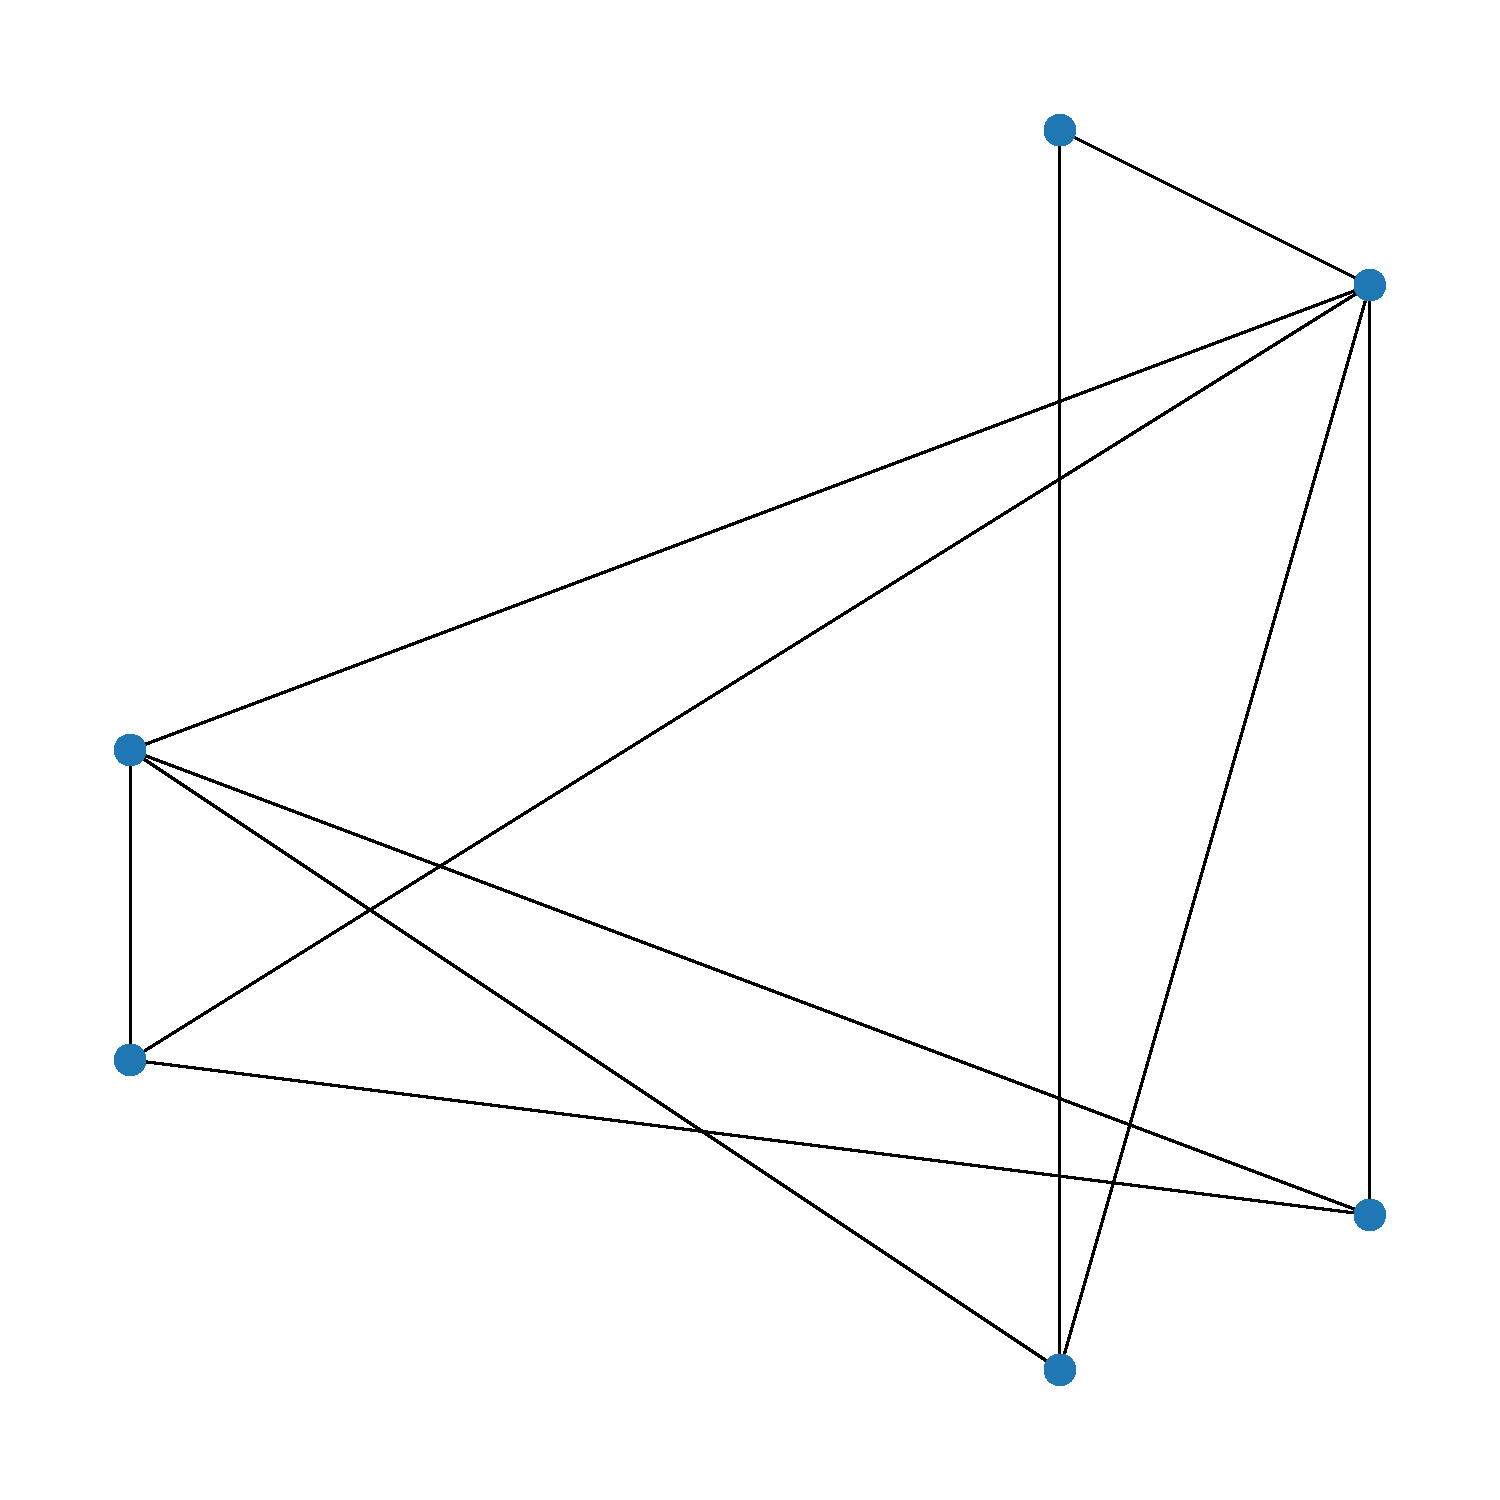
\includegraphics[width=\linewidth]{figures/algo_progress/original_default_graph.pdf}
        \caption{Straight-line graph}
        \label{fig:def_0}
    \end{subfigure}
    \begin{subfigure}{0.32\linewidth}
        \centering
        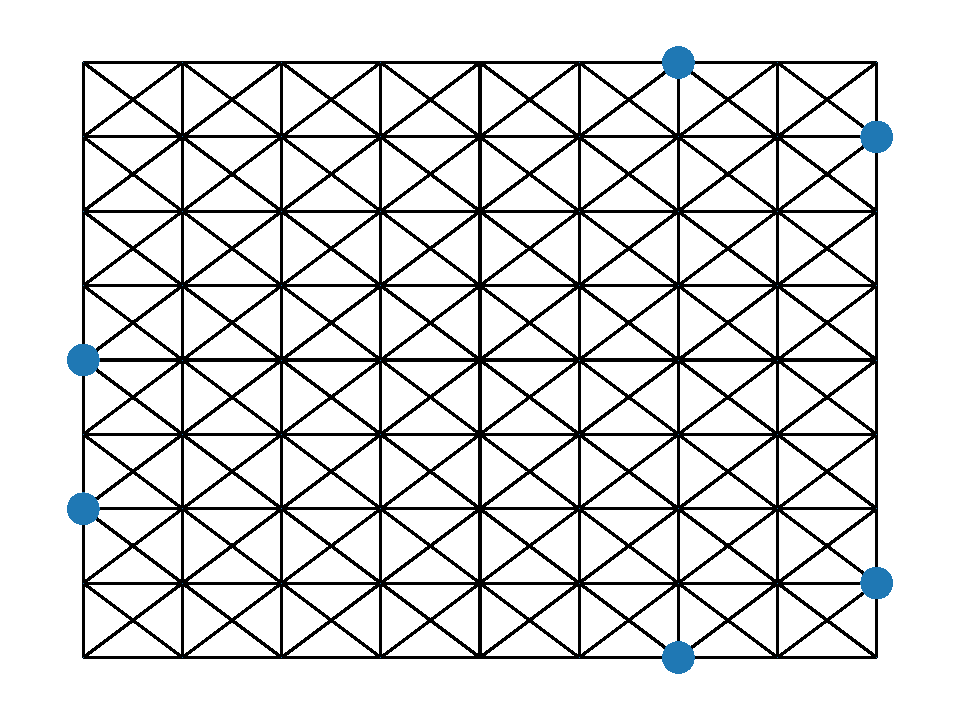
\includegraphics[width=\linewidth]{figures/algo_progress/default_graph_1-0.pdf}
        \caption{Generated grid-graph}
        \label{fig:def_1}
    \end{subfigure}
    \begin{subfigure}{0.32\linewidth}
        \centering
        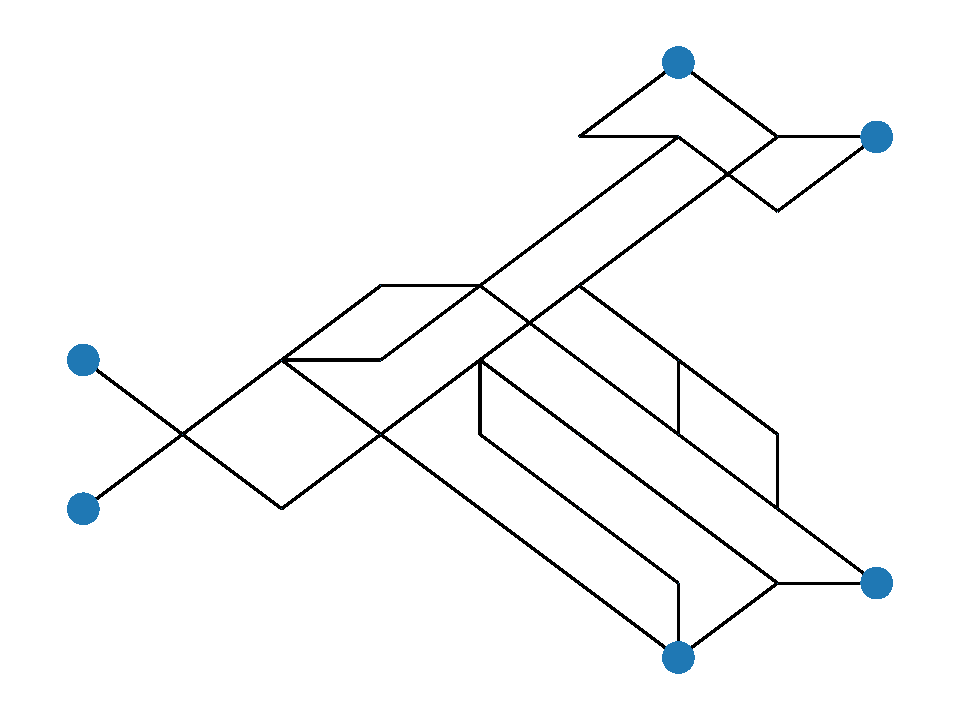
\includegraphics[width=\linewidth]{figures/algo_progress/default_graph_1-50.pdf}
        \caption{Grid after 50 iterations}
        \label{fig:def_2}
    \end{subfigure}
    \begin{subfigure}{0.32\linewidth}
        \centering
        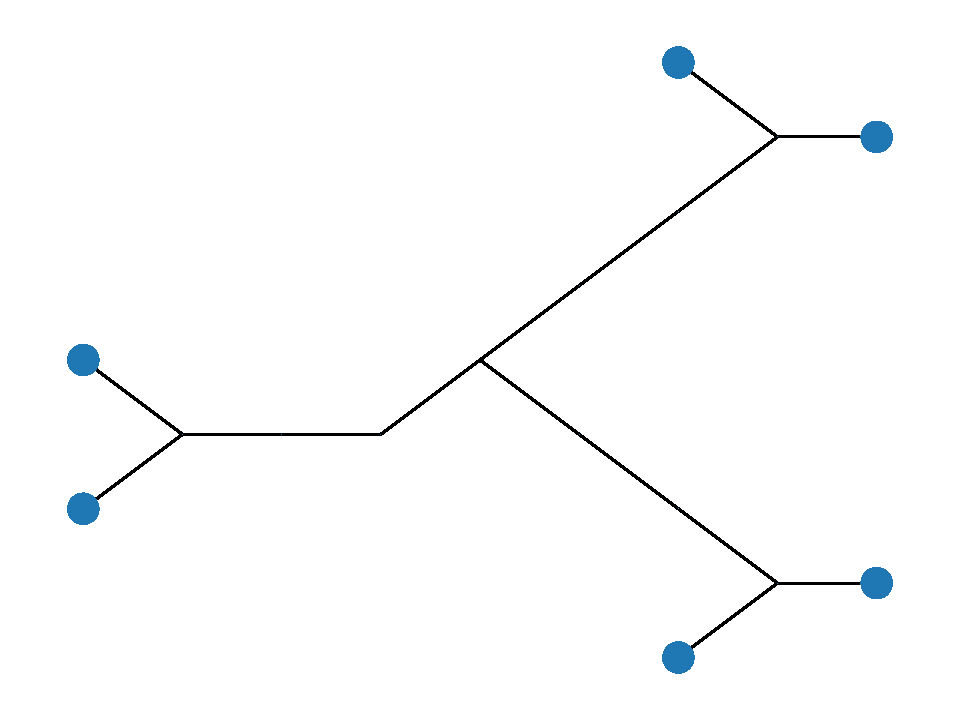
\includegraphics[width=\linewidth]{figures/algo_progress/without_clean_default.pdf}
        \caption{Finished calculation}
        \label{fig:def_3}
    \end{subfigure}
    \begin{subfigure}{0.32\linewidth}
        \centering
        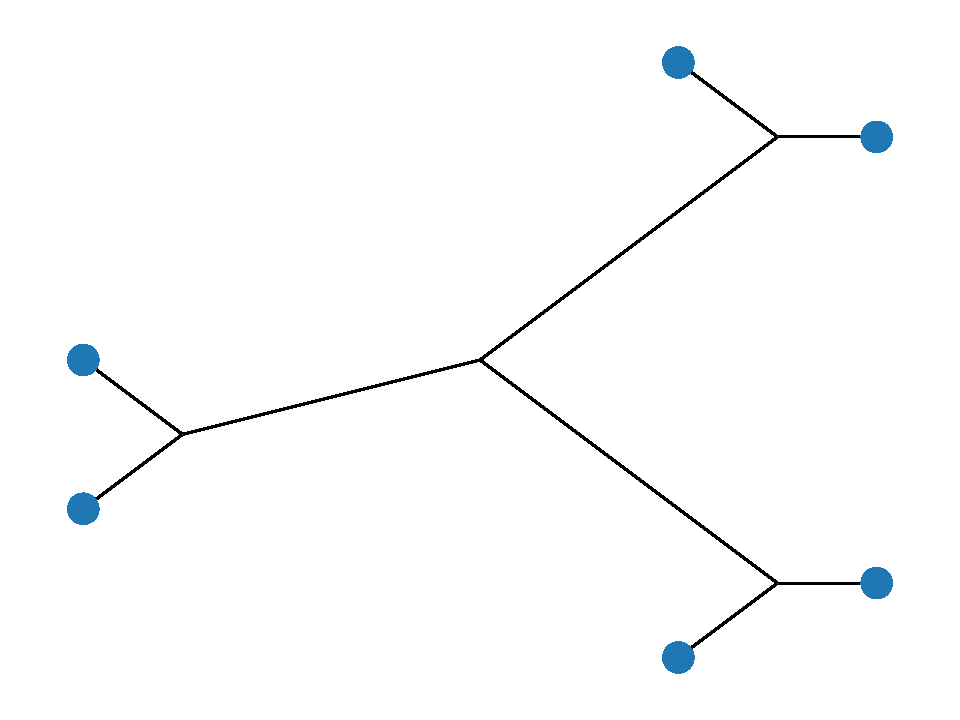
\includegraphics[width=\linewidth]{figures/algo_progress/unused_nodes_default.pdf}
        \caption{Removed unused nodes}
        \label{fig:def_4}
    \end{subfigure}
    \begin{subfigure}{0.32\linewidth}
        \centering
        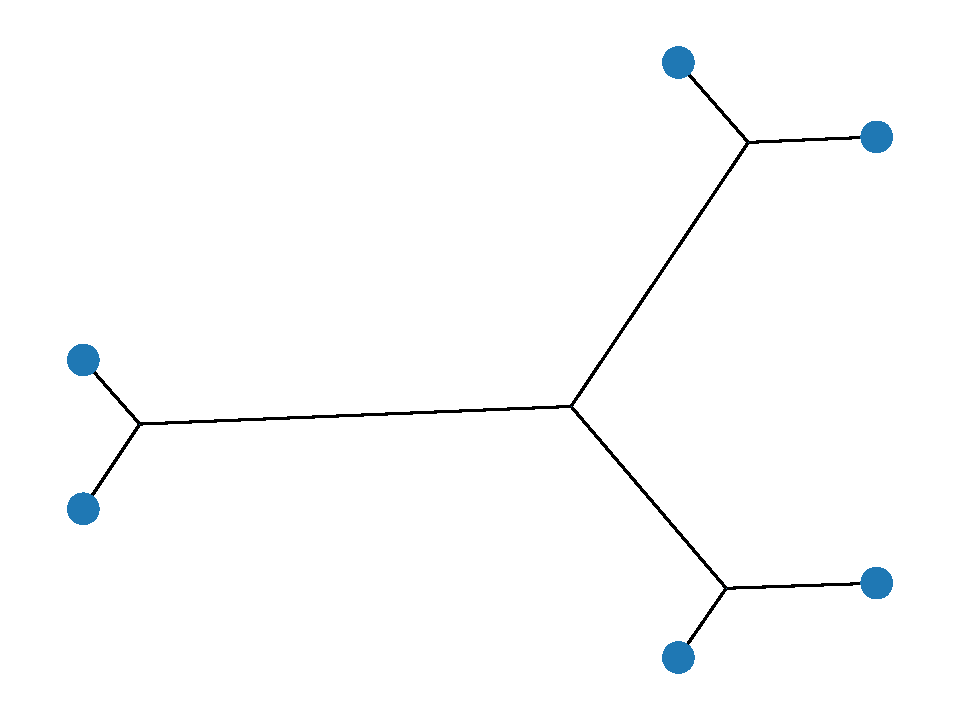
\includegraphics[width=\linewidth]{figures/algo_progress/fermat_default.pdf}
        \caption{Fermat point calculation}
        \label{fig:def_5}
    \end{subfigure}
  \caption{This figure visualizes the different steps our algorithm takes to reach a solution. \subref{fig:def_0} is the original graph as it is defined in the JSON file. Figure \subref{fig:def_1} is the grid graph built to calculate the Steiner points. \subref{fig:def_2} is the grid after 50 iterations; easy to spot is how the number of edges has shrunk. Figure \subref{fig:def_3} is the finished graph with the lowest cost. The solution from \subref{fig:def_3} still has unnecessary nodes, which are deleted by step \subref{fig:def_4}. The last step \subref{fig:def_5} is the Fermat point calculation that determines the position of the Steiner points.}
  \label{fig:default_combined}
\end{figure}

\section{Algorithm}
\label{sec:alogrithm}
We used a combination of the second and third approaches as our basis and expanded upon it. Our work is available on GitHub \cite{algortihm}.

% ************************************************************************
\begin{algorithm}
\caption{Physarium Steiner bundling}\label{psb_algorithm}
    \begin{algorithmic}
        \Require Graph $G = (V,E)$, with $V$ as terminals, viscosity value, initial flow
        
        \While {savedNetwork is None}
            \State Setup grid-environment $env$
            \State initialize edge conductivity
            \State calculate node and edge weights
            \For {outerIteration}
                \For {$edge \in edgeList$}
                    \State Initialize composite cost using \autoref{eqn:composite_cost_eqn}
                    \State Calculate the neighbor factor
                \EndFor
            
                \For {innerIteration}
                    \State Choose sink and source node using \autoref{eqn:probability_eqn}
                    \State Calculate pressure using \autoref{eqn:poisson_eqn}
        
                    \For {$edge \in edgeList$}
                        \State Calculate flux using \autoref{eqn:flux}
                        \State Update conductivities using \autoref{eqn:conductivity_update_eqn}
        
                        \If{edge conductivity < $\epsilon$}
                            \State Remove edge
                        \Else
                            \State Update edge conductivity
                            \State Calculate the neighbor factor
                        \EndIf
                    \EndFor
        
                    \If{Early inner iteration stop}
                        \For{$terminal \in terminalNodeList$}
                            \State Check terminal connections
                        \EndFor
        
                        \For{$edge \in edgeList$}
                            \State Calculate total edge cost
                            \State Check Steiner connections
                        \EndFor
                    \EndIf
                
                \EndFor
        
                \For{$edge \in edgeList$}
                    \State Calculate total edge cost
                    \State Check Steiner connections
                \EndFor
        
                \State \textbf{return} totalEdgeCost, steinerConnections
                
            \EndFor
        
            \If{toalEdgeCost $<$ currentEdgeCost}
                \State Current network becomes savedNetwork
            \EndIf
        
            \If{savedNetwork is None}
                \State innerIteration $*$ 1.5
                \State outerIteration $+$ number of cores $+$ 4
            \EndIf
            
        \EndWhile    
    \end{algorithmic}
\end{algorithm}
% ************************************************************************

%%%%%%%%%%%%%%%%%%%%%%%%%%%%%%%%%%%%%%%%%%%%%%%%%%%%%%%%%%%%%%%%%%%%%%%%

%%%%%%%%%%%%%%%%%%%%%%%%%%%%%%%%%%%%%%%%%%%%%%%%%%%%%%%%%%%%%%%%%%%%%%%%
\subsection{Building the Grid Graph}
\label{sec:grid_graph}
The first thing we did was build our grid graph generation, as the other papers did not mention how they got their grid graph. We calculated the dimensions of the graph by subtracting the minimal $x$ and $y$ values from the maximal values. The subtraction prevents unnecessary node creation if the graph does not begin at the origin of the coordinate system. 

In the next step, each node is connected to all nodes in a radius of $\sqrt{2}$. This means that a node in the center of the grid has eight connections, allowing for a more straightforward Steiner point calculation. With this method, we created the grid graph in \autoref{fig:def_1} from the original graph \autoref{fig:def_0}.

Not all graphs have node weights, so we set our weights and edge cost. The node weight is the sum of the euclidean distances between the node and each terminal. 

\begin{equation}
    \label{eqn:node_weights}
    w_i = \sum\limits_{j=0}^{|T|}  \sqrt{(x_{t_j} - x_i)^2 + (y_{t_j} - y_i)^2}
\end{equation}

The edge cost is the weights of its start and end node divided by the number of edges. 

\begin{equation}
    \label{eqn:edge_cost}
    c_{i,j} = \frac{w_i + w_j}{|E|}
\end{equation}
%%%%%%%%%%%%%%%%%%%%%%%%%%%%%%%%%%%%%%%%%%%%%%%%%%%%%%%%%%%%%%%%%%%%%%%%

%%%%%%%%%%%%%%%%%%%%%%%%%%%%%%%%%%%%%%%%%%%%%%%%%%%%%%%%%%%%%%%%%%%%%%%%
\subsection{Physarium Calculation}
\label{sec:physarium_calculation}
After the grid graph is created and the edges get their associated cost, the Physarium calculation can start. It begins by initializing the conductivity and the composite cost according to \autoref{eqn:conductivity_eqn} and \autoref{eqn:composite_cost_eqn}. 
In the next step, the sink node is chosen by \autoref{eqn:probability_eqn}, and the pressure is calculated with \autoref{eqn:poisson_eqn}. 
Next, the flux is calculated by \autoref{eqn:flux}, and the conductivity of each edge is updated using \autoref{eqn:conductivity_update_eqn}. If the conductivity is smaller than the threshold, it will be cut from the graph. In \autoref{fig:def_2} and \autoref{fig:def_3}, two iteration steps are illustrated, one after 50 iterations and the other at the end of the Physarium calculation.

These calculations continue until the iterations stop is reached. However, the graph can stabilize before implementing an early iteration stop if the graph does not change for several iteration steps. The exact number of steps is the number of edges in the grid graph before any calculations are performed. It also checks that each terminal has only one connection and that no node has more than three. The total edge cost is calculated and checked against the currently best-cost network. If the new cost is lower, the new network is saved, and the following calculation is executed until the outer iteration limit is reached. 
%%%%%%%%%%%%%%%%%%%%%%%%%%%%%%%%%%%%%%%%%%%%%%%%%%%%%%%%%%%%%%%%%%%%%%%%

%%%%%%%%%%%%%%%%%%%%%%%%%%%%%%%%%%%%%%%%%%%%%%%%%%%%%%%%%%%%%%%%%%%%%%%%
\section{Optimization}
\label{sec:optimization}

A significant part of our work was to optimize and test the algorithm as much as possible, as Sun et al. \cite{sun_fast_2016} only tried their algorithm with 100 vertices, and our goal was to solve at least a 25 x 25 grid in an acceptable amount of time.
The first step was, in addition to removing the edges, to remove all nodes that no longer had any connections to the rest of the grid, as they served no purpose. As in the next iteration step, they no longer influence the network. Other improvements include the integration of initialization of conductivity into the edge creation, a faster grid creation algorithm, and multi-threading of the main algorithm. 

Nevertheless, during our initial tests, we discovered that the outer and inner iteration limits are the main reason for the poor performance. They could be reduced significantly and still produce a good approximation. The first step we took was to implement an early iteration stop if there are no longer edges removed for several iterations. The number of iterations required for the stop is the number of edges in the graph at the start of the algorithm. We calculate a 10x10 grid graph from 18.843 seconds to 4 seconds with these optimizations.

Our algorithm runs in $O\left(T_0 \cdot \left(n \cdot e + T_i\left(n^3\right)\right)\right)$, where $n = |V|$ number of nodes, $e = |E|$ number of edges, $T_0$ the number of outer iterations and $T_i$ the number of inner iterations.
%%%%%%%%%%%%%%%%%%%%%%%%%%%%%%%%%%%%%%%%%%%%%%%%%%%%%%%%%%%%%%%%%%%%%%%%

\newpage

%%%%%%%%%%%%%%%%%%%%%%%%%%%%%%%%%%%%%%%%%%%%%%%%%%%%%%%%%%%%%%%%%%%%%%%%
\begin{figure}[H]
  \centering
  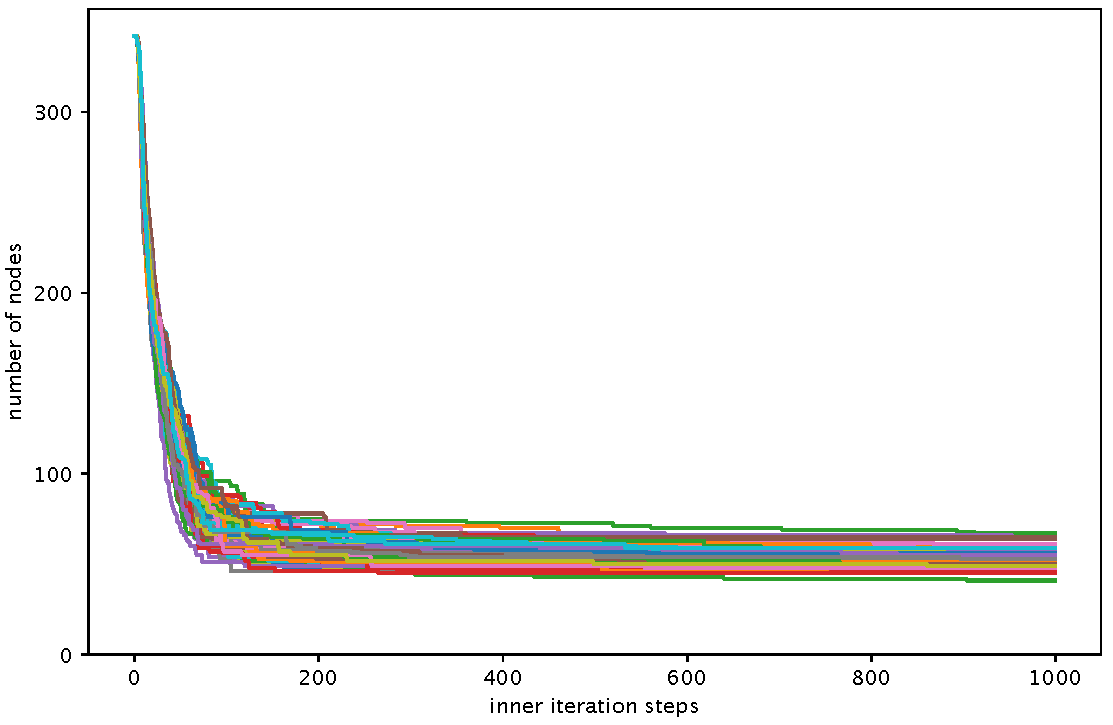
\includegraphics[width=1\linewidth]{figures/inner_iteration.pdf}
  \caption{The number of nodes in a 340 nodes test graph for the first 1000 inner iteration steps. The outer iteration was set to 100, meaning our algorithm calculated the test graph 100 times, and each line is one outer iteration. Easy to spot is the rapid decline in nodes in the first 100 iterations. This inside can be used for the optimal iteration bound.}
  \label{fig:inner_plots}
\end{figure}

\subsection{Inner Iteration Bound}
\label{sec:inner_iteration}

As one can see in \autoref{fig:inner_plots}, the most significant reduction of nodes takes place in the first 100 steps of the iteration. The size and structure of the graph have no impact on this result. We concluded that a lower bound for the inner iteration could improve the performance significantly, and the result would still be an acceptable Steiner tree approximation. As a sweet spot for the internal iteration limit, we found the inner iteration bound should be $|E|^{3}$. We added an exception for graphs where $|E|^{3}$ is smaller than 2000, as the iteration speed for those small graphs is fast either way, and the chance of a non-optimal Steiner tree is significantly reduced.
%%%%%%%%%%%%%%%%%%%%%%%%%%%%%%%%%%%%%%%%%%%%%%%%%%%%%%%%%%%%%%%%%%%%%%%%

%%%%%%%%%%%%%%%%%%%%%%%%%%%%%%%%%%%%%%%%%%%%%%%%%%%%%%%%%%%%%%%%%%%%%%%%
\begin{figure}[H]
  \centering
  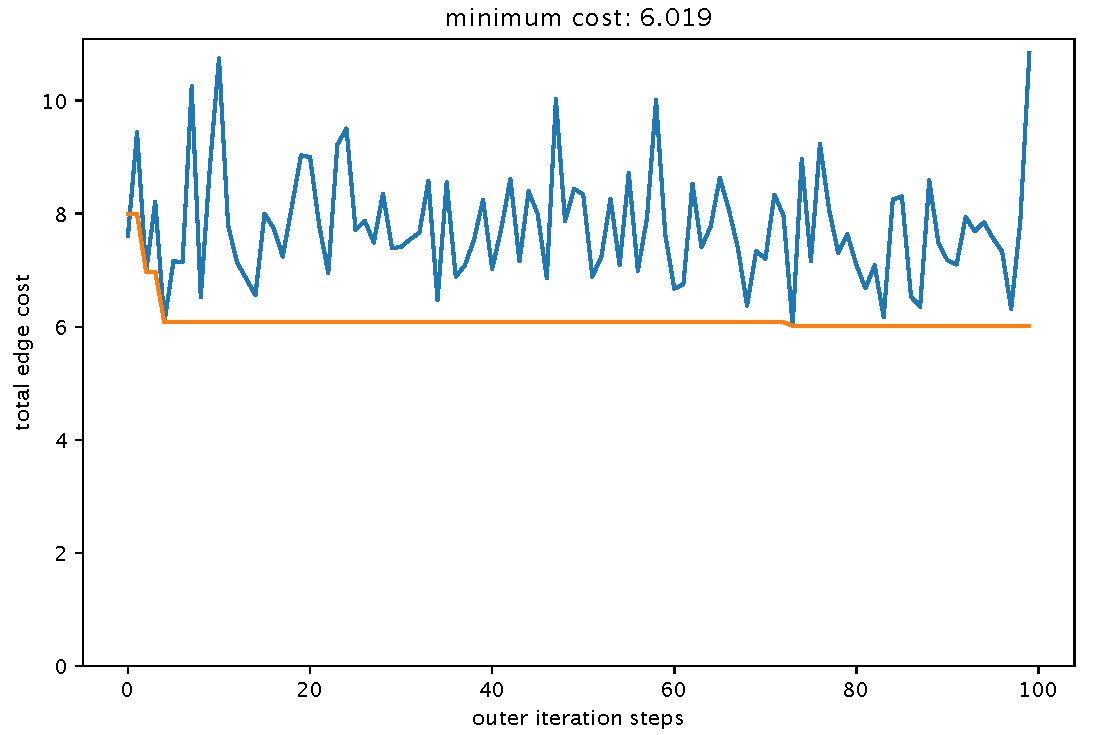
\includegraphics[width=1\linewidth]{figures/outer_iteration.pdf}
  \caption{This graph shows how the cost of the graph can reach a minimum early on and that it only improves slightly. The current minimum is displayed as the orange line, and the calculated minimum is the blue line.}
  \label{fig:outer_plots}
\end{figure}

\subsection{Outer Iteration Bound}
\label{sec:outer_iteration}

Initially, the number of outer iterations was determined by multiplying the x and y-axis. However, as the \autoref{fig:outer_plots} suggests, many external iterations are unnecessary. The algorithm only needs a few iterations to find a network shorter than the minimal spanning tree. From that point onward, the gains for running more iterations diminished rapidly as the length of the graph only shortened by a tiny amount. These gains are even further reduced by our post-processing method, which is discussed in the next section.
The number of outer iterations is the number of processing cores on the machine the algorithm is running. To ensure that the approximation calculated a good Steiner tree, we check if the total length is smaller than the minimal spanning tree. If that is not the case, we again start the outer iterations, only this time, we multiply the inner iteration bound by 1.5.
%%%%%%%%%%%%%%%%%%%%%%%%%%%%%%%%%%%%%%%%%%%%%%%%%%%%%%%%%%%%%%%%%%%%%%%%

%%%%%%%%%%%%%%%%%%%%%%%%%%%%%%%%%%%%%%%%%%%%%%%%%%%%%%%%%%%%%%%%%%%%%%%%
\section{Graph Cleaning and Post-Processing}
\label{sec:cleaning_and_processing}

% ************************************************************************
\begin{table*}[tb]
  \centering
  \setlength\tabcolsep{5pt} % adjust white space inside table
  \caption{
    \label{tab:cost}
    This table displays the network cost with the minimal spanning tree, the optimized approximation bound, and the approximation with high outer and inner iteration bounds. The time is for the lower approximation and the higher approximation. For the calculation, an Apple MacBook Air M1 was used.
  }  
  \begin{tabular}{c || c c c c c c}
    \toprule
     & \textbf{MST} & \textbf{low app.} & \textbf{high app.} & \textbf{ratio} & \multicolumn{2}{c}{\bfseries time} \\
     \hline
    3\_nodes & 2.000 & 1.337 & 1.337 & 1.000 & - & - \\
    5\_nodes & 4.000 & 2.314 & 2.314 & 1.000 & - & - \\
    9\_nodes & 8.000 & 5.155 & 4.962 & 1.039 & - & - \\
    default & 5.000 & 3.546 & 3.303 & 1.074 & - & - \\
    paper\_graph & 8.000 & 5.444 & 5.184 & 1.050 & - & - \\
    25x25\_10n\_30e & 5.000 & 4.254 & 4.032 & 1.055 & - & - \\
    10x10\_10n\_30e & 9.000 & 6.748 & 5.595 & 1.206 & - & - \\
    15x15\_15n\_30e & 14.000 & 13.272 & 11.987 & 1.107 & 25:39 & 1:57:33 \\
    15x15\_10n\_40e & 5.000 & 5.941 & 5.345 & 1.111 & 00:06 & 04:37 \\
    10x10\_10n\_30e & 5.000 & 6.230 & 5.755 & 1.083 & 00:03 & 03:08 \\
    \bottomrule
  \end{tabular}
\end{table*}
% ************************************************************************

When the graph calculations are finished, and a graph is found, the graph still needs to be cleaned, as there are still unnecessary nodes left, and the Steiner points are not at their correct position, as seen in \autoref{fig:def_3}.

So the first step is to remove unused nodes. The removal of the nodes is done by starting at the terminals or Steiner points and searching along the remaining edges for nodes that only have two connections until either a Steiner node or another terminal is reached. If the unused nodes are removed, the graph looks link \autoref{fig:def_4}.
The most important part of the post-processing is the calculation of the coordinates of the Steiner points. The computation works by utilizing the Fermat point calculation already mentioned in \autoref{sec:fermat_point}. As the points for the analysis can be Steiner points, we iterate through each point until the position does not change, and we archive a stable graph. An example of the Fermat point calculation can be seen in \autoref{fig:def_5}.

After post-processing, the approximation ratio we archived was 1.024, which indicates an excellent approximation quality. We calculated it by comparing our optimized approximation calculation against an approximation where we set the outer and inner iteration bounds to a value ten times as high. Our results for different synthetic graphs and calculation time can be seen in \autoref{tab:cost}.
%%%%%%%%%%%%%%%%%%%%%%%%%%%%%%%%%%%%%%%%%%%%%%%%%%%%%%%%%%%%%%%%%%%%%%%%

%%%%%%%%%%%%%%%%%%%%%%%%%%%%%%%%%%%%%%%%%%%%%%%%%%%%%%%%%%%%%%%%%%%%%%%%
\section{Path Visualisation}
\label{sec:path_visualisation}

\begin{figure}[t]
  \centering
  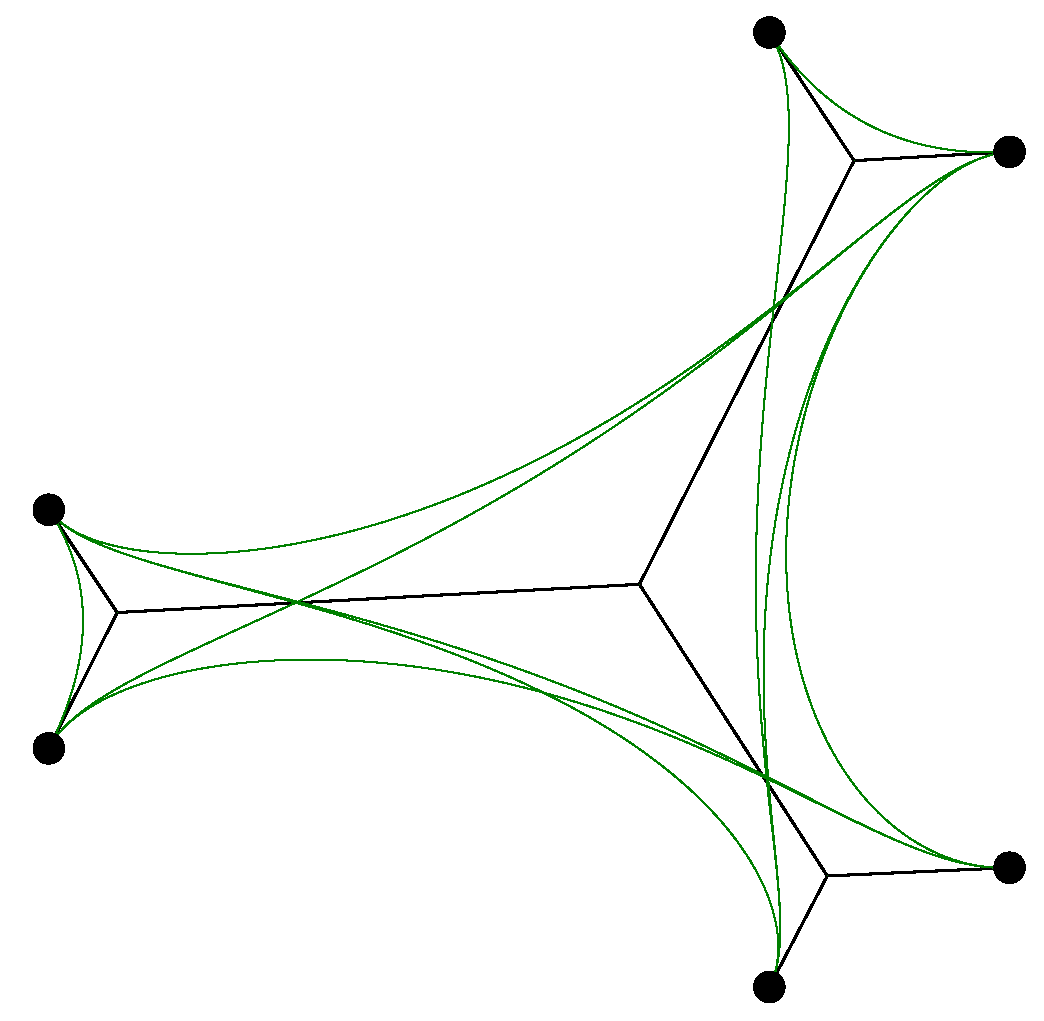
\includegraphics[width=0.6\linewidth]{figures/default_bezier+steiner.pdf}
  \caption{To better picture how the bundling works, we visualized the underlying Steiner tree and the B\'{e}zier curves in green. In the final plot, only the green edges will be visible.}
  \label{fig:default_bezier_steiner}
\end{figure}

After the post-processing cleaned the graph of unnecessary nodes and edges, only the approximated Steiner tree is left. The Steiner tree then routes the original paths along its edges. This skeletal structure gives us the ideal basis for bundling the actual paths. An example of the result can be seen in \autoref{fig:default_bezier_steiner}. The first bundling option we chose was to use the Steiner points as control points for a B\'{e}zier curve plot of the paths. This results in a bundle that is flexible in its representation and allows for a dynamic flow. In addition to the Steiner points as control points, we implemented a smoothing factor that enables the control points to be set on the edges of the tree. With each factor increase, the number of control points increased twofold.
%%%%%%%%%%%%%%%%%%%%%%%%%%%%%%%%%%%%%%%%%%%%%%%%%%%%%%%%%%%%%%%%%%%%%%%%

%%%%%%%%%%%%%%%%%%%%%%%%%%%%%%%%%%%%%%%%%%%%%%%%%%%%%%%%%%%%%%%%%%%%%%%%
\section{Graph Data and Experiments}
\label{sec:testing}

A big part of our work focused on testing and dialing the best parameters for a good approximation result. As our algorithm was still too slow for real-world graphs, we wrote a program to generate random graphs of any size and any possible combination of nodes and edges. This random graph generation enables us to test increasingly larger and more complex graphs starting from small 3x3 grid graphs up to 25x25 grid graphs. We discovered that the density of the graph significantly impacts the running time, which can even go so far that our algorithm can find no graph if the density is too high, as no Steiner tree can be created. This could be mitigated by increasing the resolution of the grid, but that would, on the other hand, impact the running time again.
We also tested alternative methods to reduce the number of nodes at the start of the approximation by running an initial calculation where the algorithm only calculates 10, 50, or 100 inner iterations. As the majority of node and edge deletions take place in these early iteration steps. Nevertheless, as our experiments have shown us, owning to the randomness of the terminal selection, it could happen that in these early stages, a crucial part of the graph network was deleted, and the following calculations could not archive a satisfactory result.
%%%%%%%%%%%%%%%%%%%%%%%%%%%%%%%%%%%%%%%%%%%%%%%%%%%%%%%%%%%%%%%%%%%%%%%%
